\documentclass[../main.text]{report}
\subsection{Ressemblence et differences entre ensembles aléatoires et nombres premiers}

Nous souhaitons maintenant comparer les groupes d'ensembles aléatoires entre eux. Pour cela, nous allons mesurer, pour chaque ensemble, le raport ${\sigma_k(n)}/{\pi(n)}$ en fonction de $n \in \mathbb{N}$, où $\sigma_k(n)$ mesure le nombre d'elements inférieurs à n.

\begin{figure}[H]
	\centering
	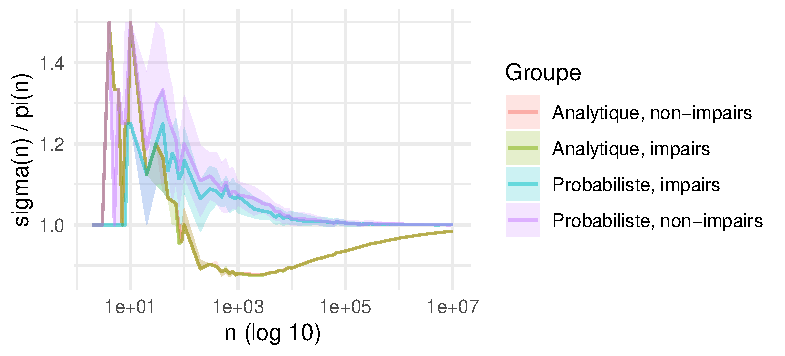
\includegraphics{comparison_all_random_sets}
	\caption{Raport entre $\sigma(x)$ et $\pi(x)$. La courbe représente la médiane de chaque groupe d'ensemble. La surface autour de la courbe montre l'espace entre les premiers et troisièmes quartiles. }
	\label{fig:comparison_all_random_sets}
\end{figure}

La figure \ref{fig:comparison_all_random_sets} montre bien que tous ces ensembles suivent la distribution de $\pi(x)$, et convergent à partir $10^3$. Il est à noter que les ensembles $Q$ (analytiques) impairs et non-impairs sont superposés. Nous voyons que le nombre d'elements dans ces ensembles est inférieur à $\pi(x)$, tandis que les ensembles $R$ (probabilistes) possèdent globalement plus d'élements. 
On observe aussi que ensembles $R$ tendent rapidement vers $pi(x)$, et montrent une plus grande dispersion. 


Nous allons maintenant mesurer à quel point ces ensembles sont différents des nombres premiers. 
%Pour cela, posons $S_n$ l'ensemble dont nous souhaitons mesurer la ressemblance à $P_n := \{p~\in~\mathbb{N}~|~p$~est~premier, p < n$\}$, et calculons alors de le cardinal de $S_n \cap P_n$. Ensuite, nous divisons ce nombre par le cardinal de $S_n$ afin d'obtenir, en pourcentage, la proportion d'élements premiers de $R_n$.
Calculons alors, pour chaque ensemble, la pourcentage de nombres premiers dans chaque ensemble, en fonction de $n$.

La figure \ref{fig:intersection_primes} montre cette proportion pour chaque groupe d'ensemble. 

\begin{figure}[H]
	\centering
	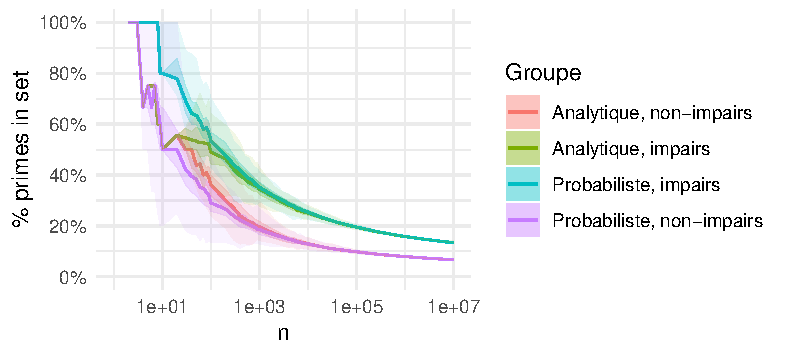
\includegraphics{intersection_primes}
	\caption{Proportion de nombres premiers dans les ensembles aléatoires en fonction de $n$, en pourcentage. La courbe représente la médiane, la surface autour de la courbe les premiers et troisièmes quartiles.}
	\label{fig:intersection_primes}
\end{figure}

À partir de $10^3$, moins de la moitié des élements des ensembles sont des nombres premiers. 
Dès $10^5$,  les nombres premiers ne représentent plus que 10\% des ensembles impairs, et 20\% des ensembles non-impairs. 
De plus, il n'y a pas de différence significative entre deux ensembles d'un même groupe dès lors que $n$ est assez grand. 